\section{Basic Extensions of the Chromosome Evolution Model}\label{sec:chromo_extensions}

In this section, we will extend the ChromEvol model in a number of ways.
First, we will examine another approach for treating chromosome number root frequencies.
This is followed by a brief example applying stochastic character mapping to chromosome evolution
models.
Then will look at jointly estimating the phylogeny and chromsome evolution,
show how to set up a BiChroM analysis, and demonstrate one way to add cladogenetic changes
to a chromosome evolution analysis.

Like before, scripts for these examples are also provided in the \RevBayes tutorial repository\footnote{\url{https://github.com/revbayes/revbayes_tutorial/tree/master/RB_Chromosome_Evolution_Tutorial/scripts}}. 
Please refer to these files to verify or troubleshoot your own scripts. 

\bigskip
\subsection{Improved Root Frequencies}\label{subsect:root_freq}

In the last example we assumed the frequency of chromosome numbers at the root of the tree
were equal. This is equivalent to assigning an extremely informative prior that all root states
are equally likely.
An alternative approach is to treat the root frequencies
as free parameters of the model and estimate them from the observed data.
In a series of unpublished simulations performed by the authors this resulted in increased accuracy of 
ancestral root chromosome numbers estimates. 


To use this approach, the \texttt{root\_frequencies} parameter must be redefined
as a stochastic node in our graphical model instead of a deterministic node.
Remove the following line from your \Rev script:
{\tt \begin{snugshade*}
\begin{lstlisting}
root_frequencies := simplex(rep(1, max_chromo + 1))
\end{lstlisting}
\end{snugshade*}}

We will instead use an uninformative flat Dirichlet prior for the root frequencies.
First, we create a vector to hold the concentration parameters for the Dirichlet
distribution. Here we set all concentration parameters to 1, which results in all
sets of probabilities being equally likely.
We then pass the vector of concentration parameters into the Dirichlet distribution
and create the stochastic node representing root frequencies.
{\tt \begin{snugshade*}
\begin{lstlisting}
root_frequencies_prior <- rep(1, max_chromo + 1)
root_frequencies ~ dnDirichlet(root_frequencies_prior)
\end{lstlisting}
\end{snugshade*}}

Next, we must specify MCMC moves for the root frequencies.
When the maximum number of chromosomes is high these parameters
can have difficulty converging.
Therefore, we use two different MCMC moves. The first is Beta Simplex move, which selects one
element of the \texttt{root\_frequencies} vector and proposes
a new value for it drawn from a Beta distribution.
The second is Element Swap Simplex move, which selects two elements
of the \texttt{root\_frequencies} vector and simply swaps their values.
{\tt \begin{snugshade*}
\begin{lstlisting}
moves[mvi++] = mvBetaSimplex(root_frequencies, alpha=0.5, weight=10)
moves[mvi++] = mvElementSwapSimplex(root_frequencies, weight=10)
\end{lstlisting}
\end{snugshade*}}
You can experiment with different weights for each MCMC move.


\medskip
\subsection{Stochastic Character Mapping of Chromosome Evolution}\label{subsub:joint_estimation}

In \RevBayes both ancestral states and stochastic character maps can be sampled from
continuous-time Markov chain (CTMC) and state-dependent speciation and
extinction (SSE) models of character evolution.
Stochastic character maps show the timing and number of transitions
along the branches of the phylogeny, so they can be particularly useful
for chromosome evolution estimates where the timing of, for example, whole genome duplication events
might be of interest. This example is performed on a non-ultrametric tree, but
the same analysis could be performed on time-calibrated trees.


We have already shown how to sample ancestral states above, and here we show
the few extra lines of \Rev code needed to sample stochastic character maps.
Stochastic character maps are drawn during the MCMC, so we need to include the
\texttt{mnStochasticCharacterMap} monitor.
{\tt \begin{snugshade*}
\begin{lstlisting}
monitors[4] = mnStochasticCharacterMap(ctmc=chromo_ctmc, filename="output/ChromEvol_maps.log", printgen=10)
\end{lstlisting}
\end{snugshade*}}
This monitor will create the \texttt{output/ChromEvol\_maps.log} file.
Just like the other log files, each row in this file represents a different sample from the MCMC.
Each column in the file, though, is the character history for a different node in the phylogeny.
The last column of the file is the full stochastic character map of the entire tree
in \textbf{SIMMAP} \citep{bollback2006simmap} format.
These can be plotted using the \textbf{phytools} R package \citep{revell2012phytools}.

After the MCMC, we can calculate the maximum a posteriori marginal, joint, or conditional
character history. This process is similar to the ancestral state summaries.
First we read in the stochastic character map trace.
{\tt \begin{snugshade*}
\begin{lstlisting}
anc_state_trace = readAncestralStateTrace("output/ChromEvol_simple_maps.log")
\end{lstlisting}
\end{snugshade*}}
Then we use the \texttt{characterMapTree} function. This generates two SIMMAP formatted files:
1) the maximum a posteriori character history, and 2) the posterior probabilities of the
entire character history.
{\tt \begin{snugshade*}
\begin{lstlisting}
characterMapTree(phylogeny, anc_state_trace, character_file="output/character.tree", posterior_file="output/posterior.tree", burnin=5, reconstruction="marginal")
\end{lstlisting}
\end{snugshade*}}
Figure \ref{fig:simmap} is an example stochastic character map of our \textit{Aristolochia} analysis plotted using \textbf{phytools}. 

\begin{figure}[h!]
\fbox{
\begin{minipage}{\textwidth}\centering
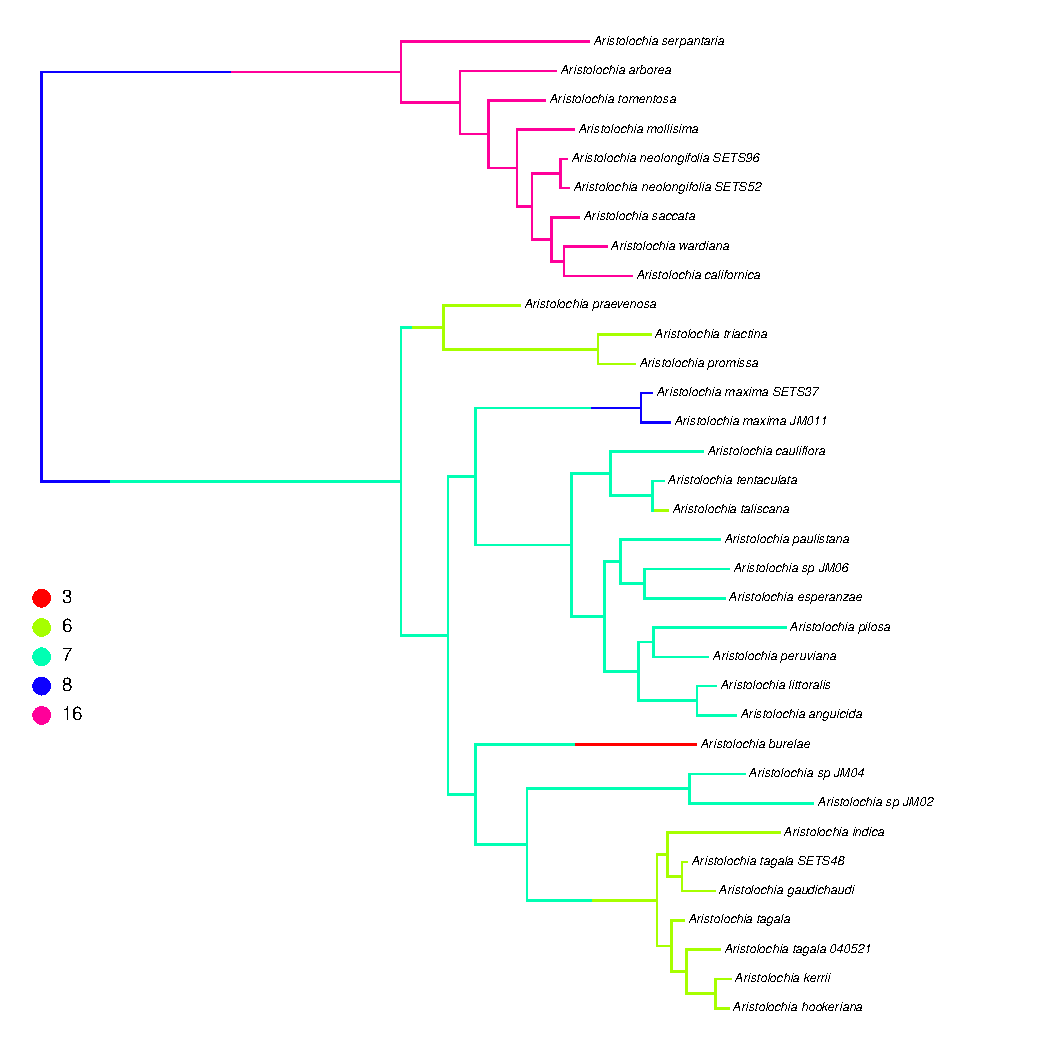
\includegraphics[width=0.92\textwidth,angle=0]{\ResourcePath figures/simmap}
    \caption{\small 
    An example of stochastic character mapping applied to chromosome number evolution using \RevBayes. Shown is the marginal maximum a posteriori chromosome evolution history of \textit{Aristolochia}
    using the simple ChromEvol analysis from Section \ref{sec:chromo_basic_analysis}.}
\end{minipage}}
\label{fig:simmap}
\end{figure}

\medskip
\subsection{Joint Estimation of Phylogeny and Chromosome Evolution}\label{subsub:joint_estimation}


In \RevBayes the chromosome evolution models can be used jointly with a model of molecular evolution 
enabling joint inference of the phylogeny and chromosome number evolution.
This enables the chromosome number analysis to take into account phylogenetic uncertainty 
and allows the chromosome numbers to help inform the phylogeny. 

Setting up a model that jointly infers chromosome evolution and phylogeny requires mostly combining
elements covered in the \textbf{Molecular Models of Character Evolution} tutorial with the
what has already been covered in Section \ref{sec:chromo_basic_analysis} of this tutorial. We will not repeat how to set up the chromosome model
component, but show what must be added to the example in Section \ref{sec:chromo_basic_analysis} above.
However, we have provided a full working example script \texttt{scripts/ChromEvol\_joint.Rev}.

\subsubsection{Reading in Molecular Data and Setting Clade Constraints}

The first major difference from the basic ChromEvol example shown above is that we must additionally
read in molecular sequence data:
{\tt \begin{snugshade*}
\begin{lstlisting}
dna_seq = readDiscreteCharacterData("data/aristolochia_matK.fasta")
\end{lstlisting}
\end{snugshade*}}
We will need some useful information about this data as well:
{\tt \begin{snugshade*}
\begin{lstlisting}
n_species = dna_seq.ntaxa()
n_sites = dna_seq.nchar()
taxa = dna_seq.names()
n_branches = 2 * n_species - 2
\end{lstlisting}
\end{snugshade*}}
Since we want to jointly infer ancestral states, we need to set an a priori
rooting constraint on our phylogeny. So here we set an ingroup and outgroup.
{\tt \begin{snugshade*}
\begin{lstlisting}
outgroup = ["Aristolochia_serpantaria", "Aristolochia_arborea", "Aristolochia_wardiana",
            "Aristolochia_californica", "Aristolochia_saccata", "Aristolochia_mollisima",
            "Aristolochia_tomentosa", "Aristolochia_neolongifolia_SETS52", "Aristolochia_neolongifolia_SETS96"]
\end{lstlisting}
\end{snugshade*}}
Here we loop through each taxon and if it is not present in the outgroup
defined above we add it to the ingroup.
{\tt \begin{snugshade*}
\begin{lstlisting}
i = 1
for (j in 1:taxa.size()) {
    found = false
    for (k in 1:outgroup.size()) {
        if (outgroup[k] == taxa[j].getSpeciesName()) {
            found = true
            break
        }
    }
    if (found == false) {
        ingroup[i] = taxa[j].getSpeciesName()
        i += 1
    }
}
\end{lstlisting}
\end{snugshade*}}
And now we make the vector of clade objects to constrain our tree topology.
{\tt \begin{snugshade*}
\begin{lstlisting}
clade_ingroup = clade(ingroup)
clade_outgroup = clade(outgroup)
clade_constraints = [clade_ingroup, clade_outgroup]
\end{lstlisting}
\end{snugshade*}}

\subsubsection{Tree Model}

We will specify a uniform prior on the tree topology, and add
a MCMC move on the topology.
{\tt \begin{snugshade*}
\begin{lstlisting}
topology ~ dnUniformTopology(taxa=taxa, constraints=clade_constraints, rooted=TRUE)
moves[mvi++] = mvNNI(topology, weight=10.0)
\end{lstlisting}
\end{snugshade*}}
Next, we create a stochastic node for each branch length.
Each branch length prior will have an exponential distribution with rate 1.0.
We'll also add a simple scaling move for each branch length.
{\tt \begin{snugshade*}
\begin{lstlisting}
for (i in 1:n_branches) {
    br_lens[i] ~ dnExponential(10.0)
    moves[mvi++] = mvScale(br_lens[i], lambda=2, weight=1)
}
\end{lstlisting}
\end{snugshade*}}
Finally, build the tree by combining the topology with the branch lengths.
{\tt \begin{snugshade*}
\begin{lstlisting}
phylogeny := treeAssembly(topology, br_lens)
\end{lstlisting}
\end{snugshade*}}

\subsubsection{Molecular Substitution Model}

We'll specify the GTR substitution model applied uniformly to all sites.
Use a flat Dirichlet prior for the exchange rates.
{\tt \begin{snugshade*}
\begin{lstlisting}
er_prior <- v(1,1,1,1,1,1)
er ~ dnDirichlet(er_prior)
moves[mvi++] = mvSimplexElementScale(er, alpha=10, weight=3)
\end{lstlisting}
\end{snugshade*}}
And also a flat Dirichlet prior for the stationary base frequencies.
{\tt \begin{snugshade*}
\begin{lstlisting}
pi_prior <- v(1,1,1,1)
pi ~ dnDirichlet(pi_prior)
moves[mvi++] = mvSimplexElementScale(pi, alpha=10, weight=2)
\end{lstlisting}
\end{snugshade*}}
Now create a deterministic variable for the nucleotide substitution rate matrix.
{\tt \begin{snugshade*}
\begin{lstlisting}
Q_mol := fnGTR(er, pi)
\end{lstlisting}
\end{snugshade*}}
Create a stochastic node for the sequence evolution continuous-time Markov chain (CTMC)
and clamp the sequence data.
Note we should have two CTMC objects in this model: one for the model of molecular evolution
and one for the model of chromosome evolution.
{\tt \begin{snugshade*}
\begin{lstlisting}
dna_ctmc ~ dnPhyloCTMC(tree=phylogeny, Q=Q_mol, branchRates=1.0, type="DNA")
dna_ctmc.clamp(dna_seq)
\end{lstlisting}
\end{snugshade*}}

\subsubsection{MCMC and Summarizing Results}

We set up the MCMC just as before, except here we
need to add a file monitor to store the sampled trees.
{\tt \begin{snugshade*}
\begin{lstlisting}
monitors[2] = mnFile(filename="output/ChromEvol_joint.trees", printgen=10, phylogeny)
\end{lstlisting}
\end{snugshade*}}
Summarizing the results of the MCMC analysis are a little different.
First we will calculate the maximum a posteriori (MAP) tree.
{\tt \begin{snugshade*}
\begin{lstlisting}
treetrace = readAncestralStateTreeTrace("output/ChromEvol_joint.trees", treetype="non-clock")
map_tree = mapTree(treetrace, "output/ChromEvol_joint_map.tree")
\end{lstlisting}
\end{snugshade*}}
Now we'll summarize the ancestral chromosome numbers over the MAP tree.
Read in the ancestral state trace:
{\tt \begin{snugshade*}
\begin{lstlisting}
anc_state_trace = readAncestralStateTrace("output/ChromEvol_joint_states.log")
\end{lstlisting}
\end{snugshade*}}
Finally, calculate the marginal ancestral states from the traces over the MAP tree.
Note that this time we have to pass both the tree trace and the ancestral state
trace to the \texttt{ancestralStateTree} function.
Since we sampled a joint distribution of ancestral state histories and trees,
we sampled some ancestral states for nodes that do not exist in the MAP tree.
Therefore the ancestral state probabilities being calculated for the MAP tree
are conditional to the probability of the node existing.
{\tt \begin{snugshade*}
\begin{lstlisting}
ancestralStateTree(map_tree, anc_state_trace, treetrace, "output/ChromEvol_joint_final.tree" burnin=0.25, reconstruction="marginal")
\end{lstlisting}
\end{snugshade*}}
Like before, we can plot the results using the \RevGadgets R package.

\bigskip

\subsection{Associating Chromosome Evolution with Phenotype: BiChroM}\label{subsect:clado_simple}


{\tt \begin{snugshade*}
\begin{lstlisting}
\end{lstlisting}
\end{snugshade*}}

\begin{figure}[h!]
\fbox{
\begin{minipage}{\textwidth}\centering
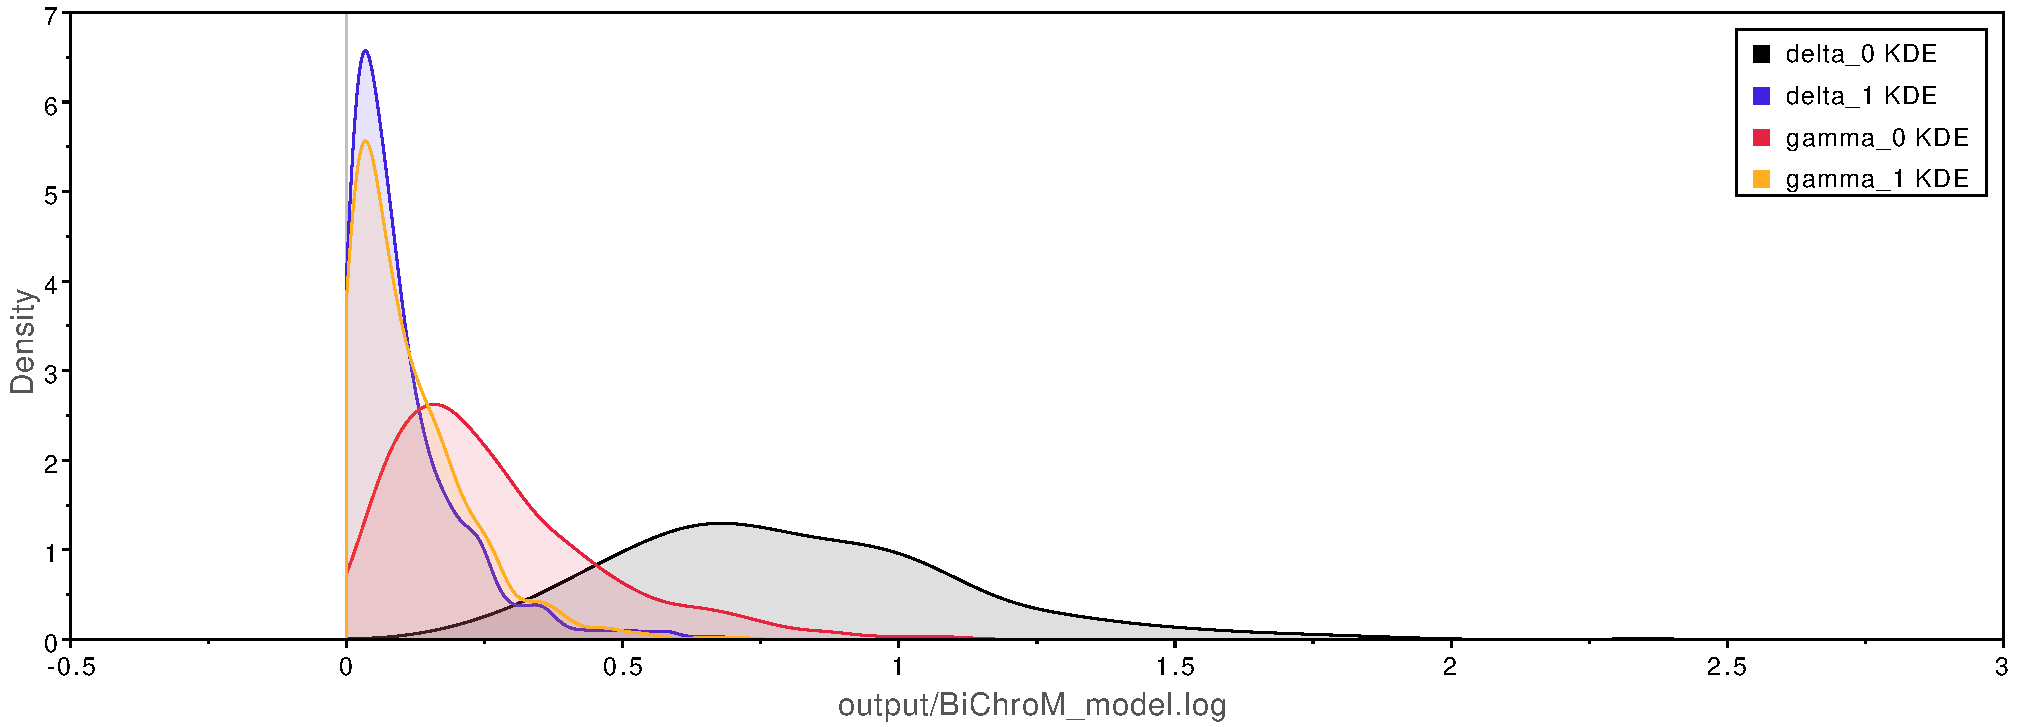
\includegraphics[width=0.92\textwidth,angle=0]{\ResourcePath figures/BiChroM_rates}
    \caption{\small The rates of chromosome gains (\texttt{gamma}) and losses (\texttt{delta}) are higher for \textit{Aristolochia}
    lineages with complex gynostemium subdivided into 5 to 24 lobes (state 0) compared
    to lineages with simple 3 lobed gynostemium (state 1).}
\end{minipage}}
\label{fig:bichrom_rates}
\end{figure}

\begin{figure}[h!]
\fbox{
\begin{minipage}{\textwidth}\centering
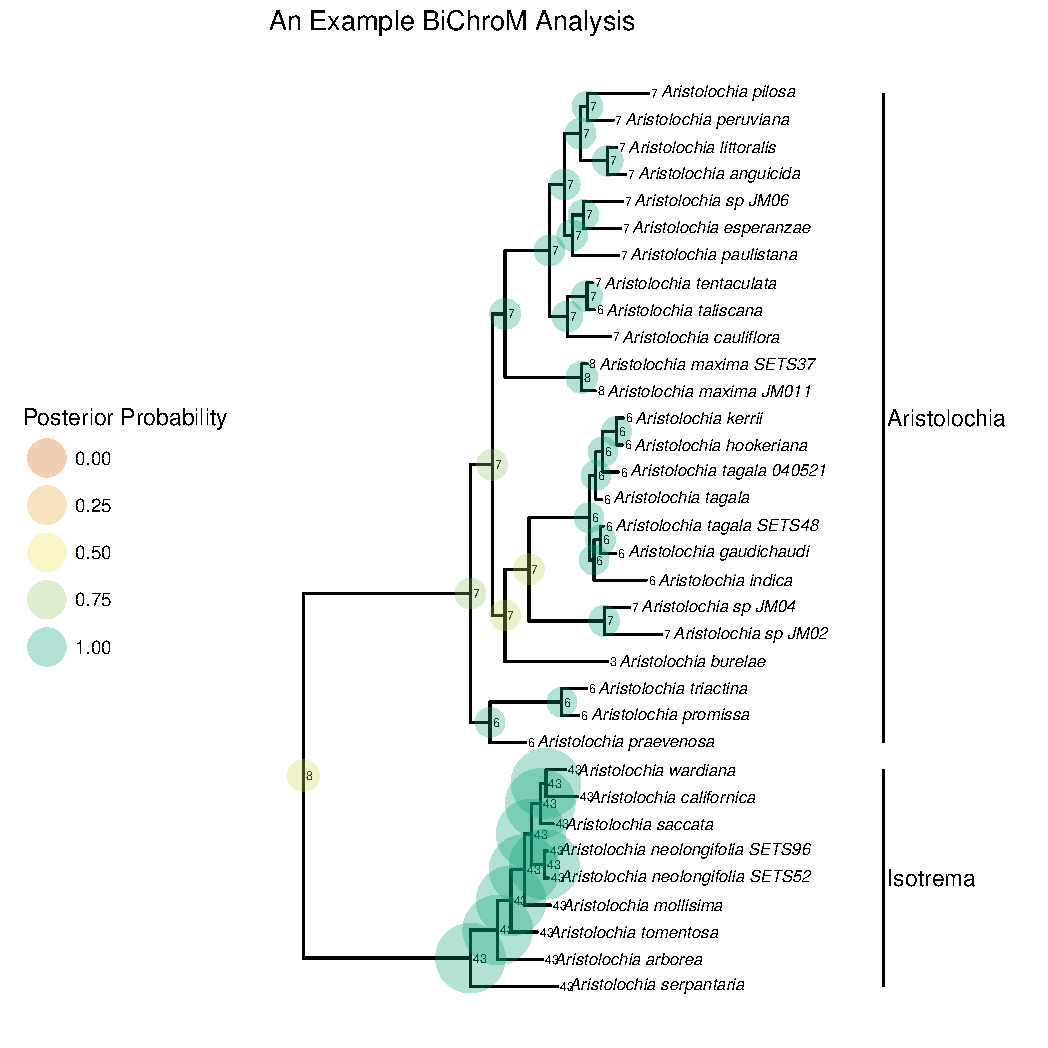
\includegraphics[width=0.92\textwidth,angle=0]{\ResourcePath figures/BiChroM}
\caption{\small Maximum a posteriori estimates of ancestral chromosome number and gynostemium morphology for \textit{Aristolochia}. States 1-26 represent the haploid number $n$ of chromosome for lineages
    with gynostemium subdivided in 5 to 24 lobes. States 27-52 represent the haploid number $n + 27$ of chromosomes 
    for lineages with simple 3 lobed gynostemium. The ancestral state for the common ancestor of all \textit{Aristolochia} had a haploid number $n = 8$ and more complex 5 to 24 lobed gynostemium. An evolutionary reduction to 3 lobes is inferred in the lineage leading to the extant Isotrema clade.}
\end{minipage}}
\label{fig:bichrom}
\end{figure}


\subsection{Incorporating Cladogenetic and Anagenetic Chromosome Changes}\label{subsect:clado_simple}


{\tt \begin{snugshade*}
\begin{lstlisting}
\end{lstlisting}
\end{snugshade*}}





\newpage
